\documentclass[11pt,compress,serif]{beamer}
%\includeonlyframes{current}

\usepackage[utf8x]{inputenc}
\usepackage[T1]{fontenc}
\usepackage[english]{babel}
% \usepackage{booktabs}
\usepackage{hyperref}
\usepackage{url}
%\usepackage{auto-pst-pdf}
%\usepackage{pst-plot}

% \usepackage{pstricks-add}

\usepackage{graphicx}
\definecolor{mygreen}{HTML}{4A7023}

\usepackage{xspace}
\usepackage{xcolor}
\usepackage{minted}
\definecolor{rulecolor}{rgb}{0.80,0.80,0.80}
\newminted{python}{frame=single,rulecolor=\color{rulecolor}, fontsize=\scriptsize}

\graphicspath{{./images/}}

\DeclareMathOperator{\Tr}{Tr}
\DeclareMathOperator{\E}{E}
\DeclareMathOperator{\Var}{Var}

% Theme
\mode<presentation>
{
    \usetheme{default}
}

\setbeamertemplate{footline}[frame number]


% Non navigation symbal
\setbeamertemplate{navigation symbols}{}

% Between section
\AtBeginSection[]
{
    %   \frame
    %   {
    %       \frametitle{Outline}
    %       \tableofcontents[currentsection]
    %   }
}

% Between subsection
\AtBeginSubsection[]
{
    %   \begin{frame}<beamer>
    %    \frametitle{Outline}
    %    \tableofcontents[currentsection,currentsubsection]
    %   \end{frame}
}


% Talk information
\author[A. Joly]{Arnaud Joly}
\title{The genesis of clusterlib \\A open source library to tame your favourite super-computer}
% \institute[Ulg]{\includegraphics[height=2cm]{logo_coul_texte_blason_cadre}}
\date{May 2015}
\subject{}
%\logo{} %change here. I used an eps file logo, you can use jpg or other format


\begin{document}
    
\frame[plain]
{
    \titlepage
}

\frame{

\frametitle{First use cases for the birth of clusterlib}
\framesubtitle{Solving supervised learning tasks, (kaggle contests?), ...}
The goal of supervised learning is to learn a function from
\structure{input}-\alert{output} pairs in order to predict the \alert{output} 
for any new \structure{input}.

\begin{footnotesize}
    \begin{columns}[b]
        \begin{column}{0.5\textwidth}
            \begin{block}{}
                \structure{A supervised learning task}
                
                \includegraphics[width=\textwidth]{forest_pruning_nolearn}
            \end{block}
        \end{column}
        
        \begin{column}{0.5\textwidth} 
            \structure{A learnt function}               
            
            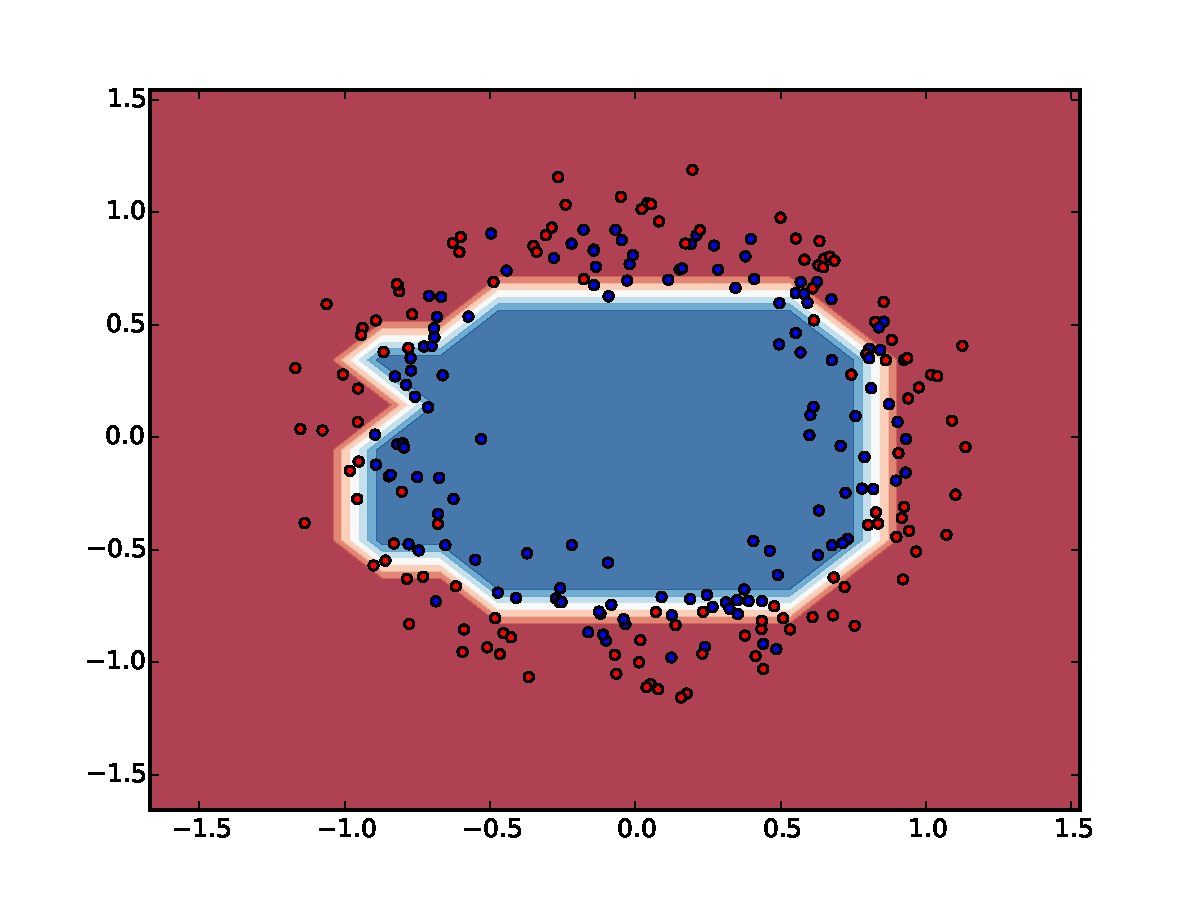
\includegraphics[width=\textwidth]{decision_tree_boundary}
            
        \end{column}
    \end{columns}
\end{footnotesize}
}

\frame{
\frametitle{Second use cases for the birth of clusterlib}
\framesubtitle{Compression of tree ensemble models}
The learnt function was a decision tree model. Nowadays instead of only one tree, 
we generate very large ensemble of randomized decision tree.
    
\begin{center}    
    \includegraphics[width=0.7\textwidth]{decision_tree_structure}
\end{center}

How to compress those models while preserving accuracy? 
\emph{L1-based compression of random forest models}
\cite{joly2012l1}
}


\frame{

\frametitle{Third use cases for the birth of clusterlib}
\framesubtitle{Multilabel classification tasks}

Many applications in text, biology or image processing where samples are associated 
to sets of labels or continuous response.

\begin{columns}[T]
    \begin{column}{0.5\textwidth}
        \begin{block}{Input $\mathcal{X}$ $800 \times 600$ pixel}
            \begin{center}
                \includegraphics[width=\textwidth]{image_anotation}
            \end{center}
        \end{block}
    \end{column}
    
    \begin{column}{0.4\textwidth}        
        \begin{block}{Output $\mathcal{Y}$ labels}
            driver, mountain, road, car, tree, rock, line, human, \ldots
        \end{block}
        
        \begin{block}{}
            If each label corresponds to a wikipedia article, then we have
            around \alert{4 million labels}.
        \end{block}
    \end{column}
\end{columns}

How to handle very high label space? \emph{Random forests with random projections of the output space 
for high dimensional multi-label classification \cite{joly2014random}}
}

\frame{
\frametitle{Time is running out}

I have huge set of experiments

\[
O(\text{\#dataset} \times  \text{\#algorithms}  \times  \text{\#parameters}) \leq O(\text{time before deadline})
\]

But, we have \alert{embarrassingly parallel tasks}. Let's use the supercomputer.
We \structure{hope} to be able  
\begin{itemize}
\item to launch easily a lot of parameter combinations;
\item to avoid launching running or queued jobs;
\item to avoid launching completed jobs.
\item to be queue scheduler agnostic (SLURM? SGE?).
\item to have few / no  dependences.
\end{itemize}
  
}

\begin{frame}[fragile=singleslide]
\frametitle{A glimpse to a supercomputer user interface (SLURM)}
\framesubtitle{How to sumit a job?}

First write a batch file \texttt{job.sh} which contain memory requirements
and what needs to be done.

\begin{verbatim}
#!/bin/bash
#
#SBATCH --job-name=job-name
#SBATCH --time=10:00
#SBATCH --mem=1000

srun hostname
\end{verbatim}

Then you can launch the job through \texttt{sbatch job.sh}.

\end{frame}

\begin{frame}[fragile=singleslide]
\frametitle{A glimpse to a supercomputer user interface (SLURM)}
\framesubtitle{How to check if a job is running?}

To check if a job is running, you can use the \texttt{squeue} command.

\begin{scriptsize}
\begin{verbatim}
$ squeue -u ajoly
JOBID PARTITION     NAME     USER  ST       TIME  NODES NODELIST(REASON)
1225128      defq wipo-20f    ajoly  PD       0:00      1 (Priority)
1225129      defq wipo-a36    ajoly  PD       0:00      1 (Priority)
...
1224607      defq wipo-a31    ajoly   R    7:39:16      1 node025
1224605      defq wipo-08d    ajoly   R    7:43:25      1 node040
1224593      defq wipo-59d    ajoly   R    8:06:33      1 node035
\end{verbatim}
\end{scriptsize}

\end{frame}


\frame{
\frametitle{Back to the checklist}

\begin{itemize}
\item Can we launch easily a lot of parameter combinations? \structure{No!}
\item Can we avoid launching running or queued jobs? \structure{No!}
\item Can we avoid launching completed jobs? \structure{No}
\item Will it work for several clusters (at least SGE, SLURM)? \structure{No}
\item Do we have to install dependencies? \structure{No}, good point! 
\end{itemize}    


}


\frame{
\frametitle{Let's not reinvent the wheel}

\begin{itemize}
\item \structure{Distributed Resource Management Application API} (DRMAA): unfortunately, it's not 
       installed on all clusters (installation require root access?).  Some packages are based
       on this: \structure{python-drma}, \structure{galaxy}, \ldots
\item \structure{Bosco} (\url{http://bosco.opensciencegrid.org/}): a compatibility layer for 
       several schedulers with similar interface to SLURM/SGE.
\item \structure{FireWorks} (\url{http://pythonhosted.org/FireWorks/}): seems pretty complete, 
      but it's much more complex than my basics needs.  It also has 6 required dependencies, among 
      them mongodb, and 7 optional dependencies. 
\end{itemize}

Arf, no suitable library on the market. At this point, I decided to write clusterlib.

}

\begin{frame}[fragile=singleslide]
\frametitle{clusterlib - How to launch a job?}

First, generate a submission script on the fly
\begin{pythoncode}
>>> from clusterlib.scheduler import submit
>>> script = submit("srun hostname", job_name="test",
...                 time="10:00", memory=1000, backend="slurm")
>>> print(script)
echo '#!/bin/bash
srun hostname' | sbatch --job-name=test --time=10:00 --mem=1000 
\end{pythoncode}

Let's launch the job
\begin{pythoncode}
>>> os.system(script)
\end{pythoncode}
    
\end{frame}

\begin{frame}[fragile=singleslide]
\frametitle{clusterlib - How to launch a tons of jobs?}
    

\begin{pythoncode}
>>> for param in range(3):
...     script = submit('./main --param %s' % param, 
                        job_name='j-%s' % param)
...     print(script)
...     # os.system(script)
... 
echo '#!/bin/bash
./main --param 0' | sbatch --job-name=j-0 --time=24:00:00 --mem=4000
echo '#!/bin/bash
./main --param 1' | sbatch --job-name=j-1 --time=24:00:00 --mem=4000
echo '#!/bin/bash
./main --param 2' | sbatch --job-name=j-2 --time=24:00:00 --mem=4000
\end{pythoncode}
        
\end{frame}

\begin{frame}[fragile=singleslide]
\frametitle{clusterlib - How to avoid re-launching queued or running jobs?}
    

\begin{pythoncode}
import os
from clusterlib.scheduler import queued_or_running_jobs
from clusterlib.scheduler import submit

if __name__ == "__main__":
    scheduled_jobs = set(queued_or_running_jobs())
    for param in range(100):
        job_name = "job-param=%s" % param
        if job_name not in scheduled_jobs:
            script = submit("./main --param %s" % param,
                            job_name=job_name,
                            backend="slurm")
            os.system(script)
\end{pythoncode}

\end{frame}

   

\begin{frame}[allowframebreaks]%in case more than 1 slide needed
\frametitle{References} 

{\footnotesize
    \bibliographystyle{apalike}
    \bibliography{references}
}
\end{frame}




\end{document}

